%!TEX root = ../thesis.tex
% створюємо розділ
\chapter{Генеративні моделі у задачах сегментації супутникових знімків}
\label{chap:gans}

У другому розділі ми розглянемо генеративні моделі, які можуть
бути застосовані для генерації штучних супутникових знімків.
Особлива увага буде приділена генеративно-змагальним нейронним
мережам. Також піде мова про вирішення задачі image-to-image translation
за допомогою GAN, а саме про архітектуру Pix2Pix та її вдосконалені версії.
Та нарешті буде описано механізм застосування генеративно-змагальних мереж
для аугментації навчальних вибірок, що має за мету вирішити проблеми, які
були описані у попередньому розділі.

\section{Різновиди генеративних моделей}

Для того, щоб наблизитись до розв'язку проблеми генерації
штучних зображень,
розглянемо наступну задачу:
нехай існує набір даних $(x_1, x_2, \dots) \in X$,
які мають невідомий розподіл $\pi$.
Ми намагаємось знайти його оцінку
$$p^* \in \arg \min\limits_{p} \mathcal{D}(\pi || p),$$
де $\mathcal{D}$ - деяка
міра близькості розподілів, яка задовольняє умови
\begin{equation*}
    \begin{cases}
        \mathcal{D}(\pi || p) \geq 0, & \pi \neq p \\
        \mathcal{D}(\pi || p) = 0,    & \pi = p
    \end{cases}
\end{equation*}

Наприклад дивергенція Йонсена-Шеннона:
\begin{equation} \label{eq:jsd}
    JSD(\pi || p) = \frac{1}{2} \int\limits_{\mathbb{R}}
    \left[
        \pi(x) \log \frac{2\pi(x)}{p(x) + \pi(x)} +
        p(x) \log \frac{2p(x)}{p(x) + \pi(x)}
        \right] dx
\end{equation}

Якщо ми зможемо знайти дану оцінку розподілу для
реальних супутникових знімків, то ми зможемо
генерувати випадкові величини з даного розподілу, які
і будуть являти собою штучні знімки. Звичайно, що
пошук по усім можливим розподілам є дуже складною задачею,
тому ми зосередимось на параметричних моделях, тобто:
$$p(x | \theta) \in \arg \min\limits_{\theta} \mathcal{D}(\pi || p_\theta),$$

Існує багато методів розв'язку подібних задач, які можна поділити
на декілька великих груп \cite{goodfellow2016nips},
що зображено на рис. \ref{fig:gen_models}.

\begin{figure}[!ht]
    \centering
    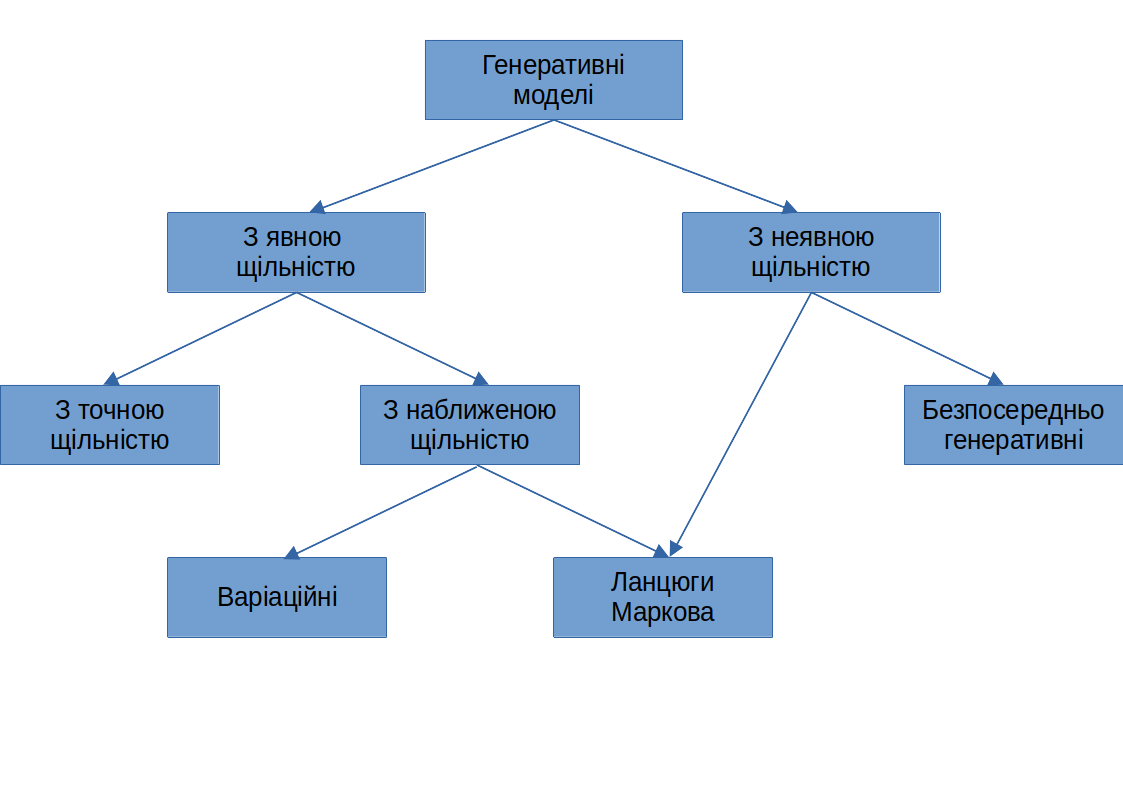
\includegraphics[width=0.9 \textwidth]{gen_models.png}
    \caption{Таксономія генеративних моделей}
    \label{fig:gen_models}
\end{figure}

Моделі з явною щільністю дозволяють обраховувати значення щільності.
Максимізація правдоподібності для даних моделей є простою,
бо являє собою просту підстановку щільності, що описує модель,
у вираз для правдоподібності. Найскладніше для даної групи
підібрати таку модель, яка зможе описувати усю складність реальних даних
і при цьому дозволить обраховувати щільність розподілу.
Тому виділяють дві стратегії:
\begin{enumerate}
    \item моделі, які гарантують можливість точного обрахунку (tractability);
    \item моделі, які ґрунтуються на обрахунку наближених значень.
\end{enumerate}

Моделі, які гарантують можливість точного обрахунку щільності, такі як
FVBN (fully visible belief networks), нормалізуючи потоки, мають перевагу у тому,
що дозволяють проводити оптимізацію безпосередньо функції
правдоподібності, проте це вимагає від них жорстких обмежень.
До того ж більшість подібних моделей виконують обрахунки послідовно,
тобто для генерації необхідно виконати декілька послідовних кроків, які
не можуть бути розпаралелині, що значно збільшує час необхідний для
генерації.

Для уникнення проблем, пов'язаних з жорсткими обмеженнями на
модель, які необхідні для точно обрахунку щільності, використовуються
моделі, які дозволяють отримувати наближені значення щільності.
Вони у свою чергу поділяються на дві групи: з детерміністичною
апроксимацією, здебільшого це автоенкодери, та зі стохастичною,
як наприклад ланцюги Маркова, машини Больцмана.

Звичайно, що і у даних підходів є суттєві недоліки.
Варіаційні автоенкодери використовують у своїй роботі
нижню границю (ELBO), яка при виборі "слабкого" апостеріорного
або ж апріорного може значно відрізнятися від справжньої
правдоподібності, що призведе до того, що розподіл генератора
та реальний розподіл будуть значно відрізнятись. На практиці
варіаційні моделі все ж здатні гарно апроксимувати правдоподібність,
проте якість згенерованих зображень є низькою. Якщо ж казати про
недоліки методів побудованих на основі ланцюгів Маркова, то
слід зазначити їх низьку швидкодію, що обумовлена як необхідністю
виконувати операції покроково, так і тим, що збіжність
дужу повільна та не має жодного методу, який би міг вказати
чи вже наявна збіжність чи потребується продовжити оптимізацію.

Концептуально іншим підходом є застосування моделей, які
не оперують щільністю або її наближеннями як такими, а
навчаються лише ґрунтуючись на тих прикладах, які надає
генератор. Тобто використовують не сам розподіл як такий, а
певні спостереження з нього. Деякі з цих моделей знову ж таки
використовують ланцюги Маркова для генерування прикладів,
здебільшого це генеративні стохастичні мережі. Але вони мають
притаманні усім ланцюгам Маркова недоліки, які були описані вище.
І на сам кінець існують моделі, які здатні безпосередньо
генерувати зображення за один крок. Найбільш відомими й поширеними з них
є генеративно-змагальні мережі, які ми розглянемо більш детально.

\section{Генеративно-змагальні мережі}

Ідея оригінального GAN  \cite{pix2pix}
полягає у тому, що ми маємо дві сутності:
генератор --- диференційовну функцію $G: Q \times \Theta_G \rightarrow X$, яка
на основі елементу з множини $Q$ (так званого латентного простору)
та параметрів $\theta_g \in \Theta_G$
генерує елемент з множин $X$; та дискримінатор
--- диференційовну функцію $D: X \times \Theta_D \rightarrow \{0, 1\}$, яка
намагається на визначити чи є елемент штучно згенерованим, чи
належить розподілу навчальних даних. Для пошуку функції
генератора та дискримінатора застосовується міні-максний функціонал якості:
\begin{equation} \label{eq:gan_criterion}
    \min\limits_{G}\max\limits_{D} \left[
        \E_{x \sim \pi} \log D(x) +
        \E_{q \sim p_{Q}} \log (1 - D(G(q))) \right],
\end{equation}
що можна уявляти як змагання між генератором і дискримінатором,
що можна побачити на наступній ілюстрації (рис. \ref{fig:gan})

\begin{figure}[h]
    \centering
    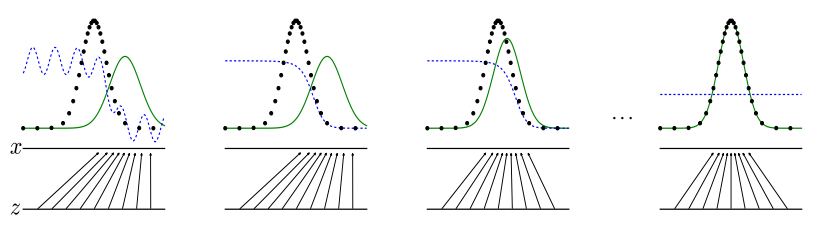
\includegraphics[width=0.75 \textwidth]{gan_distribution.png}
    \caption{Ілюстрація ідеї GAN \cite{goodfellow2014generative}.
        Зеленим позначено розподіл генератора,
        синім --- дискримінатора,
        чорними точками --- реальних даних}
    \label{fig:gan}
\end{figure}

Окремим питанням, яке заслуговує на увагу, є питання про те,
а чи дійсно у результаті розв'язку цієї задачі ми отримаємо
генератор, розподіл якого дорівнює розподілу реальних даних.
Для того, щоб переконатися у цьому доведемо дві важливі теореми.

\begin{theorem}[Гудфелоу \cite{goodfellow2014generative}]
    Для фіксованого генератора $G$ з розподілом $p_G(x)$
    оптимальним дискримінатором $D^*(x)$ є:
    \begin{equation*}
        D^{*}(x) = \frac{\pi(x)}{\pi(x) + p_G(x)}.
    \end{equation*}
\end{theorem}
\begin{proof}
    Запишемо цільову функцію:
    \begin{equation*}
        \min\limits_{G}\max\limits_{D} \left[
            \E_{x \sim \pi} \log D(x) +
            \E_{q \sim p_{Q}} \log (1 - D(G(q))) \right]
    \end{equation*}
    Генератор, за припущенням є фіксованим, тож ми можемо перейти
    від математичного сподівання по латентному просторі до математичного сподівання
    розподілу генератора $p_G(x)$.
    \begin{equation*}
        \min\limits_{G}\max\limits_{D} \left[
            \E_{x \sim \pi} \log D(x) +
            \E_{x \sim G(x)} \log (1 - D(x)) \right]
    \end{equation*}
    Наступним кроком розпишемо математичні сподівання та
    властивостями визначених інтегралів:
    \begin{equation*}
        \min\limits_{G} \int\limits_X \max\limits_{D}
        \left( \pi(x) \log D(x) +
        p_G(x) \log (1 - D(x)) \right) dx
    \end{equation*}
    Розглянемо умову екстремум для виразу під
    знаком максимуму і отримаємо:
    \begin{gather*}
        \frac{\partial}{\partial D(x)}
        \left( \pi(x) \log D(x) +
        p_G(x) \log (1 - D(x)) \right) = \\
        = \frac{\pi(x)}{D(x)} - \frac{p_G(x)}{1 - D(x)} = 0
    \end{gather*}
    І виразивши $D(x)$ остаточно отримаємо:
    \begin{equation*}
        D^{*}(x) = \frac{\pi(x)}{\pi(x) + p_G(x)}
    \end{equation*}
\end{proof}

\begin{theorem}[Гудфелоу \cite{goodfellow2014generative}]
    Глобальний мінімум критерію \eqref{eq:gan_criterion} досягається
    тобі і тільки тоді, коли розподіли генератора $p_G$ та реальних даних
    однакові. При цьому значення критерію дорівнює $-\ln 4$.
\end{theorem}
\begin{proof}
    Підставимо оптимальний дискримінатор у критерій~\eqref{eq:gan_criterion}.
    \begin{equation*}
        \min\limits_{G} \left[
            \E_{x \sim \pi} \log \frac{\pi(x)}{\pi(x) + p_G(x)} +
            \E_{q \sim p_G} \log \frac{\pi_G(x)}{\pi(x) + p_G(x)}
            \right]
    \end{equation*}
    Тепер помножимо і поділимо кожен дріб на 2 та використаємо властивість
    логарифмів та математичного сподівання від константи.
    \begin{equation*}
        \min\limits_{G} \left[
            \E_{x \sim \pi} \log \frac{2 \pi(x)}{\pi(x) + p_G(x)} +
            \E_{q \sim p_G} \log \frac{2 \pi_G(x)}{\pi(x) + p_G(x)}
            \right] - \ln 4
    \end{equation*}
    Вираз у дужках є нічим іншим як дивергенцією Йонсена-Шеннона \eqref{eq:jsd}.
    Вона приймає мінімальне значення $0$ тоді і тільки тоді, коли
    розподіли дорівнюють один одному. І, відповідно, значення критерію
    у випадку рівності $0$ мінімуму буде дорівнювати $-\ln 4$.
\end{proof}

Підсумовуючи, генеративно-змагальні мережі мають наступні
переваги над іншими моделями:
\begin{enumerate}
    \item Можливість паралельної генерації,
          що забезпечує швидкість роботи навченої моделі.
    \item На генератора накладається мало обмежень, що дає можливість
          вибору широко класу архітектур.
          Це є перевагою порівняно з машинами Больцмана,
          які допускають лише певні класи  ймовірнісних розподілів,
          а також щодо потоків, що нормалізують, які вимагають, щоб генератор
          мав зворотнє відображення, а розмірність латентного простіру
          дорівнювала розмірності даних.
    \item Не використовуються ланцюги Маркова з усіма їх
          недоліками, як у машинах Больцмана та генеративних стохастичних мережах.
    \item Генеративна мережа, оптимізація якої була збіжною, точно наближає
          розподіл реальних даних, а не використовує нижні чи верхні
          оцінки, як це у випадку з автоенкодерами.
    \item Якість зображень, які генеруються за допомогою GAN,
          здебільшого вища за інші моделі.
\end{enumerate}

Саме ці моменти і обумовлюють вибір саме генеративно-змагальних
мереж для генерації штучних супутникових знімків, і, як наслідок,
аугментації навчальних вибірок.

\section{GAN у задачах image-to-image translation}

\begin{figure}[ht]
    \centering
    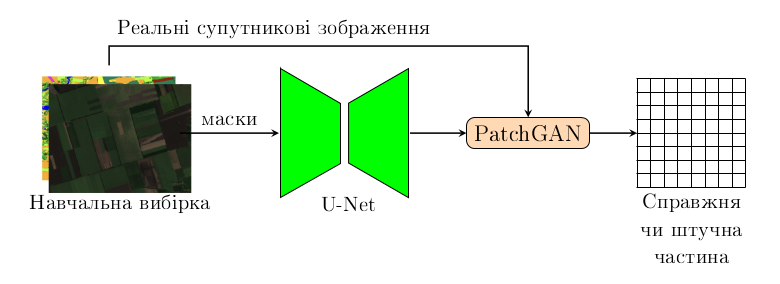
\includegraphics[scale=0.5]{pix2pix.png}
    \caption{Архітектура Pix2Pix у застосуванні до супутникових знімків}
    \label{fig:pix2pix}
\end{figure}

\section{Перспективи застосування GAN для генерації штучних супутникових знімків}

\begin{figure}[ht]
    \centering
    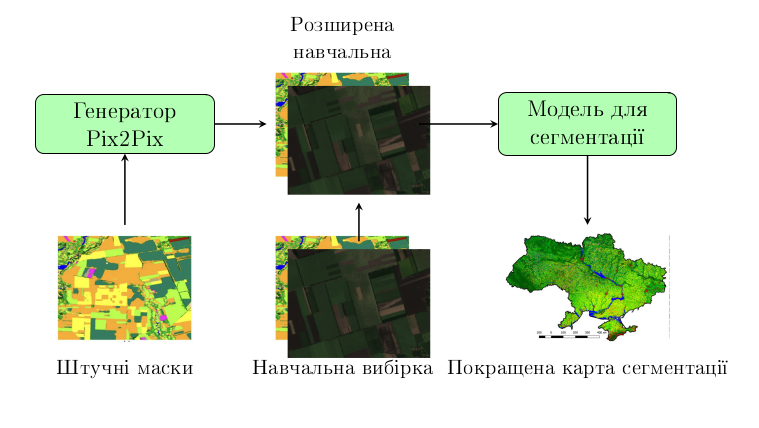
\includegraphics[scale=0.5]{pipline.png}
    \caption{Процес аугментації наборів даних супутникових знімків за допомогою Pix2Pix}
    \label{fig:pipline}
\end{figure}

\chapconclude{\ref{chap:gans}}